\documentclass[11pt, a4paper, oneside]{report}
\usepackage{mathtools}
\usepackage{amsfonts}
\usepackage{minted}
\usepackage{booktabs}
\usepackage[UKenglish]{babel}
\usepackage[en-GB,showdow]{datetime2}
\usepackage{csquotes}
\usepackage{hyperref}
\usepackage{imakeidx} \makeindex
\usepackage[
sorting=none,
hyperref=true,
backend=biber,
style=numeric,
backref=true
]{biblatex}
\addbibresource{references.bib}
\usepackage{todonotes}
\usepackage{pdfpages}
\usepackage{glossaries} \makeglossaries
\usepackage{graphicx}
\usepackage{framed}
\usepackage{dsfont}
\usepackage{caption}
\usepackage{parskip}



\newglossaryentry{term}{ name={term}, description={``a
    word or expression that has a precise meaning in some uses or is
    peculiar to a science, art, profession, or
    subject'\autocite{dictionary:_term_defin_term} --- here text
    analysts have capitalised on the generalisation of ``term'to
    include subcomponents or aggregations of words} }




\begin{document}

% \frontmatter
\begin{titlepage}
  \centering
  \vspace*{2.5cm}
  {\Huge Text Analytics}\\
  \vspace{1.5cm}
  {\Large Jason Peter Cairns}\\
  \vspace{1.5cm}
  Supervised by Chris Wild\\
  \vspace{1.5cm}
  \begin{figure}[h]
    \centering
    
\includegraphics[scale=0.4]{img/logo.jpg}
  \end{figure}
  \vspace{1cm}
  Bachelor of Science (Honours)\\
  Department of Statistics\\
  The University of Auckland\\
  New Zealand
\end{titlepage}

\listoftodos

% \begin{abstract}

% \end{abstract}

\chapter*{Acknowledgements}
\label{cha:acknowledgements}

\tableofcontents
\addcontentsline{toc}{chapter}{Listings}
\renewcommand\listoflistingscaption{List of source codes}
\listoflistings
\addcontentsline{toc}{chapter}{Tables}
\listoftables
\addcontentsline{toc}{chapter}{Figures}
\listoffigures

% \mainmatter
\chapter{Introduction}
\label{cha:introduction}

\section{Intention}
\label{sec:intention}

Text Analytics serves to glean insights from a body of text. Within the
broad category of text analytics, we seek to answer questions about
what the text is communicating, what is felt about it, and how this
information is structured. In this dissertation, we demonstrate the
creation of a user-friendly program to perform text analytics
functions using modern R with the Shiny web application framework. In
a literate style, we illustrate top-down the structure of such a
program, as well as the data structures and computational processes
that have established their value for such a program.\todo{should this
  be an abstract?}
  
\section{Background: Text Analytics (incl. examples)}
\label{sec:backgr-text-analyt}
\subsection{common functions: sentiment, summarisation, scoring}
Text Analytics is comprised of a variety of processes and techniques
to extract information from text. The text almost always requires some
initial processing. Some of the following functions have proven
utility, and are expanded upon in \autoref{cha:text-analyt-backgr};

\begin{itemize}
\item Sentiment: In order to answer what emotions are conveyed in a
  text, sentiment analysis is commonly performed. The technique yields
  some measure of what is represented in an emotional sense by the
  text, with a range different methods and their associated outputs
  allowing for different forms of the analysis. Sentiment analysis
  won't pick up the subtle nuances that a human reader would, but
  generally gives reasonable output over the extent of a text.
\item Associated Words: The meaning of a text is dependent on the
  structure between and within words. Looking at how words are
  associated, through correlation, common sequences, visualisation of
  sections, etc.,\ allow for a clear high-level assessment of the
  associations between words. The higher level not only saves
  individual efforts, but can demonstrate any emergent properties
  inherent to a text, in a way that a direct reading won't necessarily
  reveal.
\item Summarisation: Automation of an executive summary, or a list of
  key words, typically falls under the purview of summarisation. The
  primary aim is to rank and select the most ``representative'' words
  or sentences from a text. A few major techniques dominate, being
  somewhat complex in nature. The results seem to be suprisingly
  representative of a text.
\item Feature Counts: The simplest quantitative measure is very often
  the most informative; from simple word counts, to selective counts
  of sentences within groups, counting features can reveal how much
  written weighting is given to various elements, aiding insight into
  content, structure, and sentiment simultaneously.
\end{itemize}

\subsection{Existing Systems}
There are several existing systems in the field of Text Analytics. The
field was initially nurtured as a sub-field of Computer Science, being
computationally-dependent in nature. More recently, there has been
increasing statistical interest. The existing systems reflect this;
most older text analytics programs were Artificial Intelligence
focussed, being experimental in nature, typically composed in lisp.
More recently, major statistical programs have been incorporating text
analytic features, with a few smaller text-analytic specific programs
appearing. SAS, SPSS, and R are all examples of major statistical
processing systems, with recent additions of text analytics
capabilities. An overview of R packages aiding in text analytics will
be given in \autoref{sec:liter-revi-exist}.

\section{Background: inZight}
\label{sec:background:-inzight}
\subsection{What iNZight is - capabilities, popularity, etc.}
\subsection{how our program fits in - shiny, inzight lite etc.}
Our program will form part of the suite of modules extending iNZight.
It provides a simple GUI interface to rapidly perform common text
analyses. The primary audience are those learning the fundamentals and
potential of text analysis and statistics, which could include
students of the traditional text analytics fields of Statistics and
Computer Science, but can and should include students of Linguistics,
Communications, Law, History, and any other text-based field. Beyond
the educational aspects of the program, it is fully functional for
practical use for general text analysis.
\section{Literature Review (existing packages in R)}
\label{sec:liter-revi-exist}

\subsection{Copy over from notes, flesh out a bit}

\subsection{Praise tidytext book, complain about the package}

\section{Scope of work}
\label{sec:scope-work}
While the total scope possible for text analytics is enormous, our
time in creating this program is not. Thus, it is essential that we
limit the scope. There are two primary areas with which we created the
limitations: Text type, and analysis type.\\

By limiting the forms of text we work with, we can spend less effort
on consideration of every single possible import and transformation
case, and more time on the actual design of analysis. The simplest
means with which to create the limitation exists in allowing only
import of particular text files --- in this case, we allow for flat
\texttt{.txt} files, as well as tabular \texttt{.csv} and
\texttt{.xlsx} files. What we do not provide (though by design leaving
open the future possibility of inclusion) is access in-program to
common text sources through their API, such as Twitter or Project
Gutenberg.\\

Through focussing on dictionary-based, rather than model-based
analyses, we have avoided much of the associated complexities. An
example of this follows. It is common to categorise words based on
their grammatical category, then use models that take this into
account. By avoiding that (again, keeping the design flexible enough
to incorporate this in the future), we have been able to get far more
functionality implemented in a shorter amount of time, with the
analyses still performing soundly. Additionally, we focus on the
general audience, as it is typically more advanced,
linguistically-trained users who would make intelligent use of such
analyses.

\chapter{Text Analytics Prolusion}
\label{cha:text-analyt-backgr}

\section{overview}
\label{sec:overview}
Most importantly, words must be extracted, serving as the basic unit
of analysis, from which more complex items may be derived.
\subsection{Explain broadness of term}
\subsection{compile glossary from terms here}
\subsection{Areas of text analytics in a data science framework}
\subsection{what we have done}
\subsection{what we haven't done}

\section{terms}
\label{sec:terms}
\gls{term}
\subsection{terms and their centrality}
\subsection{generalisation: n-grams, sentences etc.}

\section{Historical Background}
\label{sec:hist-backgr}

\subsection{computer science vs statistics - reflection in data science}

\section{Processing}
\label{sec:processing}

\subsection{why process}
\subsection{stopwords, lemmatisation etc.}
\subsection{modelling vs db joins - more info in notes}

\section{scores \& statistics}
\label{sec:statistics}

\subsection{why compute scores \& statistics}
\subsection{scoring - tf-idf, word count}
\subsection{Suggestions for further research - more on the statistics of words}
\subsection{recount the book of John text analysis}

\section{Sentiment}
\label{sec:sentiment}

\subsection{why sentiment}
\subsection{Process of sentiment}
\subsection{sentiment modelling vs db joins}
\subsection{our implementation and why}
\subsection{reviews}
\subsection{issues}

\section{Summarisation}
\label{sec:summarisation}

\subsection{why compute summarisations}
\subsection{lexrank, textrank - include notes on lexrank}
\subsection{other methods}
\subsection{reddit bot example}

\section{what we didn't do (yet)}
\label{sec:what-we-didnt}

\subsection{topic modelling}
\subsection{Term correlation}
\subsection{modelling based on linguistic features}

\section{Visualisation}
\label{sec:visualisation-1}

\subsection{talk about score vs structure}
\subsection{complain about tag clouds}
\subsection{talk about ggpage}
\subsection{discuss our experimentations with some alternative visualisations}
\chapter{Program Structure \& Development}
\label{cha:program-structure}

\subsection{why R}
\subsection{Why Shiny}
\subsection{why tidyverse}
\subsection{Git}
\subsection{possible future: datatables, futures, etc.}
\subsection{why functional}
\subsection{Why lossless data}

\section{Program Architecture}
\label{sec:program-architecture-1}

\subsection{Why structure it like it has been}
\subsection{make graph of architecture}
\subsection{Describe package and package creation}
\subsection{following three sections copy and paste from the notes - buffing up as necessary}
\subsection{include screenshots}

\section{Preparation}
\label{sec:import}
The first step in all text analysis is to import the text data and
wrangle it into a data structure suitable for statistical analysis.

\subsection{Importing}
\label{sec:importing}

Text must first be brought in from an outside source to be useful for
the program. The import functions are such that all text from
different files exist in dataframes of equivalent structure. The
primary differences are that each row of an imported \texttt{.txt}
file corresponds to a single line, whereas each row of an imported
tabular file corresponds to the row of the tabular file. Importantly
for tabular files, the column of the text intended for analysis must
be given the header of ``text'' prior to import. This condition will
be relaxed later.-

\subsubsection{Import .txt}

The following is the simple function used in the import of \texttt{.txt} files:


\inputminted[frame=lines,fontsize=\scriptsize,xleftmargin=\parindent,linenos]{R}{R/import-txt.R}
\captionof{listing}{Import txt\label{lst:import-txt}}


\subsubsection{Import .csv}

CSV is a plaintext tabular format, with columns typically delimited by
commas, and rows by new lines. A particular point of difference in the
importation of tabular data and regular plaintext is that the text of
interest for the analysis should be (as per tidy principles) in one
column, with the rest being additional information that can be used
for grouping or filtering. Thus, additional user input is required, in
the specification of which column is the text column of interest. The
following function is effectively just a wrapper around

\inputminted[frame=lines,fontsize=\scriptsize,xleftmargin=\parindent,linenos]{R}{R/import-csv.R}
\captionof{listing}{Import csv\label{lst:import-csv}}

\subsubsection{Import Excel}

Unfortunately, much data exists in the Microsoft Excel format, but
this must be catered for. As tabular data, it is treated equivalently
to csv, with a wrapper around \mintinline{r}{readr::read_excel()}

\inputminted[frame=lines,fontsize=\scriptsize,xleftmargin=\parindent,linenos]{R}{R/import-excel.R}
\captionof{listing}{Import excel\label{lst:import-excel}}

\subsubsection{Import Wrapper for Arbitrary Number of Files}

To have just one function required to import files, we define two
functions; one that imports any file, and one making use of it to
import multiple files. The import of multiple files is no trivial
task; the program must shape them in such a way that they retain
identification, and fit into the same datastructure together.

The base wrapper function takes in the filename, and other relevent
information, handling the importation process. It also stamps in the
name of the document as a column.

The base file import is generalised to multiple files with a multiple
import function: this will be our sole import function

\inputminted[frame=lines,fontsize=\scriptsize,xleftmargin=\parindent,linenos]{R}{R/import-files.R}
\captionof{listing}{Import files\label{lst:import-files}}

\subsection{Object Preparation}

From the imported files, we work at transforming their representations
into a lossless and efficient data structure that any analysis can
make use of. Our solution to the essential constraint of losslessness
is to separate and ID by each word in a dataframe. To do this, we take
the line ID, the sentence ID, then the word ID, producing a dataframe
that takes the following form:

  \begin{table}[h]
    \centering
   
  \begin{tabular}{rrrl}
    line\_id & sentence\_id & word\_id & word\\
    \toprule
    1 & 1 & 1 & the\\
    1 & 1 & 2 & quick\\
    2 & 1 & 3 & brown\\
  \end{tabular}  
  \caption{Primary data structure format}\label{tab:data-base}
\end{table}

The reason for the ID columns is the preservation of the structure of
the text; If required, the original text can be reconstructed in
entirety, sans minor punctuation differences. The following function
automatically formats any data of the format returned by the initial
import functions.

\inputminted[frame=lines,fontsize=\scriptsize,xleftmargin=\parindent,linenos]{R}{R/text-prep.R}
\captionof{listing}{Prepare text\label{lst:text-prep}}

\subsection{Filtering}

Filtering of text is implemented directly with the
\mintinline{r}{dplyr::filter()} function, directly in the server of
the shiny app. Filtering can take place multiple times throughout an
analysis. The program is flexible enough such that after some initial
analytics have been done in the insight layer, preparation can be
returned to and the text can be filtered on based on features seen in
the analytics.

\subsection{Lemmatisation}

Lemmatisation is effectively the process of getting words into
dictionary form. It is a very complex, stochastic procedure, as
natural languages don't follow consistent and clear rules all the
time. Hence, models have to be used. Despite the burden, it is
generally worthwhile to lemmatise words for analytics, as there are
many cases of words not being considered significant, purely due to
taking so many different forms relative to others. Additionally,
stopwords work better when considering just the lemmatised form,
rather than attempting to exhaustively cover every possible form of a
word. \href{https://github.com/trinker/textstem/}{textstem} is an R
package allowing for easy lemmatisation, with it's function
\mintinline{r}{lemmatize_words()} transforming a vector of words into their
lemmatised forms (thus being compatible with \mintinline{r}{mutate()} straight
out of the box). We have the lemmatisation in this program managed
completely by this single function in the server end of the shiny app.
The package Udpipe was another option, but it requires downloading
model files, and performs far more in depth linguistic determinations
such as parts-of-speech tagging, that we don't need at this point.
It is worth noting that, like stopwords, there are different dictionaries
available for the lemmatisation process, but we will use the default,
as testing has shown it to be the simplest to set up and just as
reliable as the rest.
\subsection{Stemming}

Stemming is far simpler than lemmatisation, being the removal of word
endings. This doesn't require as complex a model, as it is
deterministic. It is not quite as effective, as the base word ending
is not concatenated back on at the tail, so we are left with word
stumps and morphemes. However, it may sometimes be useful when the
lemmatisation model isn't working effectively, and textstem provides
the capability with \mintinline{r}{stem_words()}. We have not
implemented this yet, as it is not as essential to an analysis when
lemmatisation is already available.

\subsection{Stopwords}\label{sec:stopwords}

We make use of dictionary-form stopwords, allowing for the input of
both developed lexicons as well as user input. Two functions compose
stopwords in the programl \mintinline{r}{get_sw()}, which gathers user
input, queries the selected lexicon and combines the two, and
\mintinline{r}{determine_stopwords()} which adds a boolean
\mintinline{r}{TRUE | FALSE} column to the input dataframe. The
following code listing defines \mintinline{r}{get_sw()} and
\mintinline{r}{determine_stopwords()}:

\inputminted[frame=lines,fontsize=\scriptsize,xleftmargin=\parindent,linenos]{R}{R/stopwords.R}
\captionof{listing}{Manage stopwords\label{lst:stopwords}}

\subsection{Formatting}\label{sec:formatting}

The final component in preparation is to format the prepared object
with the correct attributes to have formatting automated. We define a
wrapper that takes all combinations of stopwords and lemmatisation
options and intelligently connects them for the ``insight column'' in
a dataframe, which the insight is performed upon. For the purpose of
standard interoperability, e.g., with ggpage, we name this column
``text''.

At the heart of this function is an \mintinline{r}{ifexp()} that
encodes the following logic involving the interaction of stopwords and
lemmatisation, to enable the correct output text based on stopword and
lemmatisation options;

\begin{table}[h]
  \centering
  \begin{tabular}{p{20mm}|p{50mm}p{50mm}}
  & Stopwords True & Stopwords False\\
  \toprule
Lemmatise True & Lemmatise, determine stopwords on lemmatisation, perform insight on lemmas sans stopwords & Lemmatise, perform insight on lemmas\\
Lemmatise False & Determine stopwords on original words (no lemmatisation), perform insight on words sans stopwords & Perform insight on original words\\
\end{tabular}
\caption{Formatting Logic for Stopwords and Lemmatisation}\label{tab:formatting}
\end{table}

Based on the combination, stopword filtering and lemmatisation take
place inside the function, defined as the following:

\inputminted[frame=lines,fontsize=\scriptsize,xleftmargin=\parindent,linenos]{R}{R/format-data.R}
\captionof{listing}{Format data\label{lst:format-data}}

\subsection{Sectioning}

Plaintext, as might exist as a Gutenberg Download, differs from more
complex representations in many ways, including a lack of sectioning
--- for example, chapters require a specific search in order to jump
to them. Here, I compose a closure that searches and sections text
based on a Regular Expression intended to capture a particular
section. Several functions are created from that. At a later date,
advanced users could be given the option to compose their own regular
expressions for sectioning.

\inputminted[frame=lines,fontsize=\scriptsize,xleftmargin=\parindent,linenos]{R}{R/section.R}
\captionof{listing}{Detect and add sections\label{lst:section}}

\subsection{Grouping}

Grouping is an essential, killer feature of our app. The
implementation is to run a \mintinline{r}{dplyr::group_by()} command
in the shiny server on the prepared object, over user-specified
groups, and all further insights and visualisations are performed
groupwise. This allows for immediate and clear comparisons between
groups.

Like filtering, after some initial analytics have been done in the
insight layer, preparation can be returned to and the text can be
grouped on based on the analytics.

\section{Insight}\label{sec:insight}

\subsection{Term Insight}\label{sec:term-insight}

\subsubsection{Term Frequency}\label{sec:term-frequency}

\inputminted[frame=lines,fontsize=\scriptsize,xleftmargin=\parindent,linenos]{R}{R/term-freq.R}
\captionof{listing}{Determine Term Frequencies\label{lst:term-freq}}

\subsubsection{n-Grams}\label{sec:n-grams}

\inputminted[frame=lines,fontsize=\scriptsize,xleftmargin=\parindent,linenos]{R}{R/get-bigram.R}
\captionof{listing}{Get bigrams functionally\label{lst:get-bigram}}

\inputminted[frame=lines,fontsize=\scriptsize,xleftmargin=\parindent,linenos]{R}{R/concat-walk.R}
\captionof{listing}{Concatenate walks\label{lst:concat-walk}}

\inputminted[frame=lines,fontsize=\scriptsize,xleftmargin=\parindent,linenos]{R}{R/concat-walk.R}
\captionof{listing}{Concatenate walks\label{lst:concat-walk}}

\begin{minted}[frame=lines,fontsize=\scriptsize,xleftmargin=\parindent,linenos]{R}
x <- c(1, 2, NA, 4, 5, NA, 7, NA)
get_bigram(x)
\end{minted}
\captionof{listing}{Bigram example\label{lst:bigram-example}}

\inputminted[frame=lines,fontsize=\scriptsize,xleftmargin=\parindent,linenos]{R}{R/get-ngram.R}
\captionof{listing}{Get n-grams\label{lst:get-ngram}}

\inputminted[frame=lines,fontsize=\scriptsize,xleftmargin=\parindent,linenos]{R}{R/ngram-freq.R}
\captionof{listing}{Get n-grams frequencies\label{lst:get-ngram-freq}}

\subsubsection{Key Words}\label{sec:key-words}

\inputminted[frame=lines,fontsize=\scriptsize,xleftmargin=\parindent,linenos]{R}{R/keywords.R}
\captionof{listing}{Determine Key Words with Textrank\label{lst:keywords}}

\subsubsection{Term Sentiment}\label{sec:term-sentiment}

\inputminted[frame=lines,fontsize=\scriptsize,xleftmargin=\parindent,linenos]{R}{R/term-sentiment.R}
\captionof{listing}{Determine Term Sentiments\label{lst:term-sentiment}}

\subsubsection{Moving Average Term Sentiment}\label{sec:moving-average-term}

\inputminted[frame=lines,fontsize=\scriptsize,xleftmargin=\parindent,linenos]{R}{R/ma-term-sentiment.R}
\captionof{listing}{Determine the Moving Average Term Sentiment\label{lst:ma-term-sentiment}}

\subsection{Aggregate Insight}\label{sec:aggregate-insight}

\subsubsection{Term Count}\label{sec:term-count}

\inputminted[frame=lines,fontsize=\scriptsize,xleftmargin=\parindent,linenos]{R}{R/term-count.R}
\captionof{listing}{Determine the term count over some aggregate\label{lst:term-count}}

\subsubsection{Key Sections}\label{sec:key-section}

\inputminted[frame=lines,fontsize=\scriptsize,xleftmargin=\parindent,linenos]{R}{R/key-aggregates.R}
\captionof{listing}{Determine the Key Sections\label{lst:key-sections}}

\subsubsection{Aggregate Sentiment}\label{sec:aggregate-sentiment}

\inputminted[frame=lines,fontsize=\scriptsize,xleftmargin=\parindent,linenos]{R}{R/aggregate-sentiment.R}
\captionof{listing}{Determine the Aggregate Sentiments\label{lst:aggregate-sentiment}}

\subsubsection{Word Correlation}\label{sec:word-correlation}

\subsubsection{Term Frequency --- Inverse Document Frequency}\label{sec:term-freq-inverse}

\subsubsection{Topic Modelling}\label{sec:topic-modelling}

\subsection{Wrapper}\label{sec:wrapper}

\inputminted[frame=lines,fontsize=\scriptsize,xleftmargin=\parindent,linenos]{R}{R/get-insight.R}
\captionof{listing}{Insight functions wrapper\label{lst:get-insight}}

\inputminted[frame=lines,fontsize=\scriptsize,xleftmargin=\parindent,linenos]{R}{R/insight-aggregate.R}
\captionof{listing}{Bind aggregate terms\label{lst:insight aggregate}}

\section{Visualisation}\label{sec:visualisation}

\subsection{Rank}\label{sec:rank}

\subsection{Score}\label{sec:score}

\subsubsection{Bar Plot}\label{sec:bar-plot}

\inputminted[frame=lines,fontsize=\scriptsize,xleftmargin=\parindent,linenos]{R}{R/barplot.R}
\captionof{listing}{Create Bar Plot\label{lst:barplot}}

\subsubsection{Word Cloud}\label{sec:word-cloud}

\inputminted[frame=lines,fontsize=\scriptsize,xleftmargin=\parindent,linenos]{R}{R/wordcloud.R}
\captionof{listing}{Create Word Cloud\label{lst:wordcloud}}

\subsection{Distribution}\label{sec:distribution}

\subsubsection{Histogram}\label{sec:histogram}

\inputminted[frame=lines,fontsize=\scriptsize,xleftmargin=\parindent,linenos]{R}{R/histogram.R}
\captionof{listing}{Create Histogram\label{lst:histogram}}

\subsubsection{Density}\label{sec:density}

\inputminted[frame=lines,fontsize=\scriptsize,xleftmargin=\parindent,linenos]{R}{R/density.R}
\captionof{listing}{Create Kernel Density Estimate Plot\label{lst:density}}

\subsubsection{Box Plot}\label{sec:box-plot}

\subsection{Structure}\label{sec:structure}

\subsubsection{Time Series}\label{sec:time-series}

\inputminted[frame=lines,fontsize=\scriptsize,xleftmargin=\parindent,linenos]{R}{R/time-series.R}
\captionof{listing}{Create Time Series Plot\label{lst:time-series}}

\subsubsection{Page View}\label{sec:page-view}

\inputminted[frame=lines,fontsize=\scriptsize,xleftmargin=\parindent,linenos]{R}{R/page-view.R}
\captionof{listing}{Create Page View Plot\label{lst:page-view}}

\subsection{Wrapper}\label{sec:wrapper-1}

\inputminted[frame=lines,fontsize=\scriptsize,xleftmargin=\parindent,linenos]{R}{R/get-vis.R}
\captionof{listing}{Create Visualisation\label{lst:get-vis}}

\section{Application}\label{sec:application}

\inputminted[frame=lines,fontsize=\scriptsize,xleftmargin=\parindent,linenos]{R}{R/app.R}
\captionof{listing}{UI and Server of Shiny Application\label{lst:app}}

\chapter{Conclusion}\label{cha:conclusion}

\section{Summary}\label{sec:summary}

\subsection{summarise successes}
\subsection{summarise failures}
\subsection{general thoughts on the topic}

\section{Recommendations}\label{sec:recommendations}

\subsection{educational potential of text analytics}
\subsection{what else remains}

\chapter{Appendix}\label{cha:appendix}

The following pages are a copy of the documentation for the R package
created as a part of this dissertation. They were automatically
generated through the Roxygen2 system.

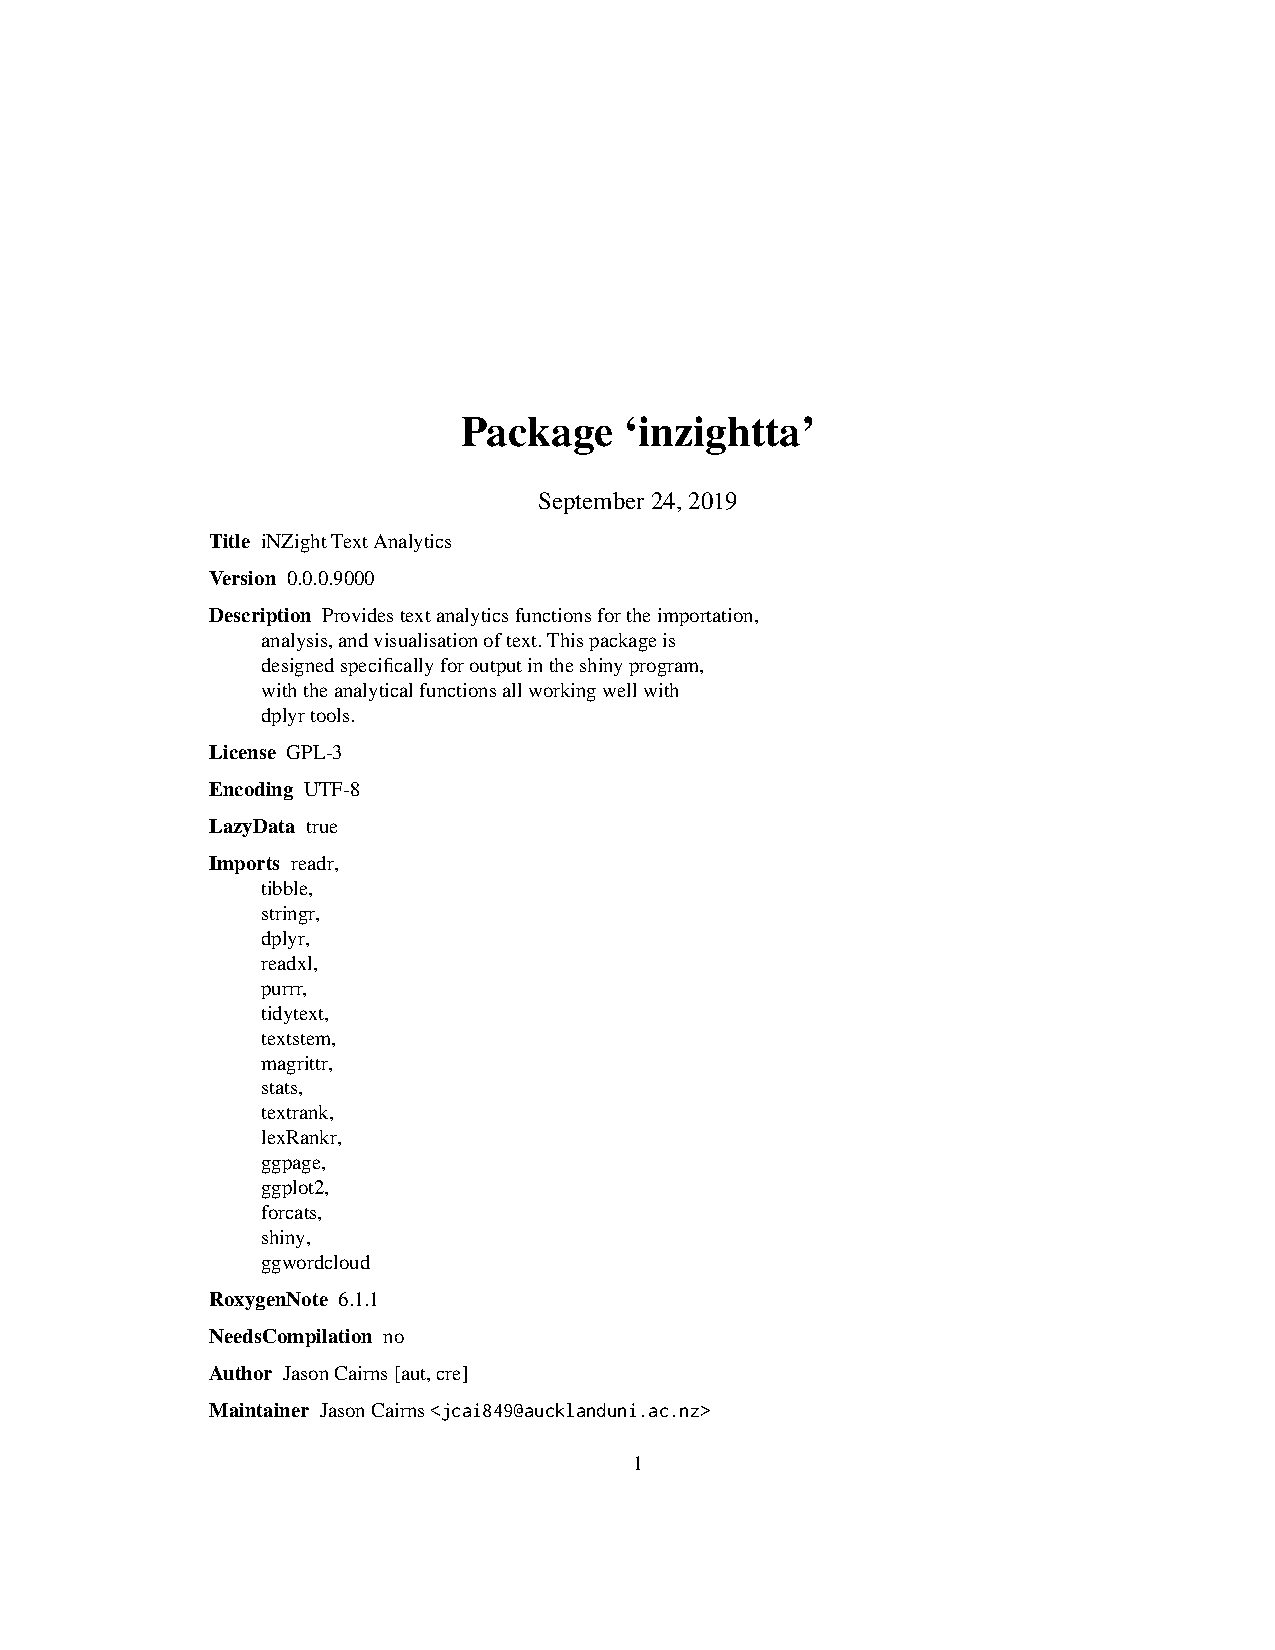
\includepdf[pages=-]{inzightta_manual.pdf}

% \backmatter
\addcontentsline{toc}{chapter}{Glossary}
\printglossaries
\addcontentsline{toc}{chapter}{Index}
\printindex
\addcontentsline{toc}{chapter}{Bibliography}
\printbibliography
\end{document}

% \begin{listing}[ht]
% \inputminted[
% frame=lines,
% framesep=2mm,
% fontsize=\footnotesize,
% linenos
% ]{R}{src/table.R}
% \caption{Example Code}
% \label{lst:test}
% \end{listing}

% \begin{table}[ht]
%   \centering
%   \input{src/output_table}
%   \caption{test table}
%   \label{tab:test}
% \end{table}